%=====================================================================
%  Proyecto 1 - Arquitectura de Computadoras
%  Programacion Vectorial en Ensamblador x86-64 (NASM/Linux)
%  Normalizador estadistico vectorizado: escalar vs AVX2
% =====================================================================
\documentclass[journal]{IEEEtran}
\usepackage[utf8]{inputenc}
\usepackage[T1]{fontenc}
\usepackage[spanish,es-tabla,es-nodecimaldot]{babel}
\usepackage{float}
\usepackage{graphicx}
\usepackage[justification=centering]{caption}
\usepackage{amsmath,amsthm,amssymb,amsfonts}
\usepackage{siunitx}
\sisetup{output-decimal-marker=,, group-separator={\,}, per-mode=symbol,
  range-phrase={~a~}, range-units=single}
\usepackage{xcolor}
\usepackage{listings}
\usepackage{tikz}
\usetikzlibrary{arrows.meta, positioning, calc, babel}
\usepackage[style=ieee, backend=biber]{biblatex}
\addbibresource{literatura.bib}
\renewcommand*{\bibfont}{\footnotesize}
\usepackage{csquotes}
\usepackage{url}
\hyphenation{en-sam-bla-dor vec-to-ri-za-cion a-cu-mu-la-dor
             re-duc-cion nor-ma-li-za-cion}
 
% ---------------------------------------------------------------------
%  Estilo para los fragmentos de codigo
% ---------------------------------------------------------------------
\definecolor{comentario}{rgb}{0.35,0.50,0.35}
\definecolor{palabra}{rgb}{0.10,0.10,0.65}
\definecolor{fondo}{rgb}{0.97,0.97,0.97}
 
\lstdefinestyle{asm}{
  language=[x86masm]Assembler,
  basicstyle=\ttfamily\scriptsize,
  commentstyle=\color{comentario}\itshape,
  keywordstyle=\color{palabra}\bfseries,
  backgroundcolor=\color{fondo},
  numbers=left, numberstyle=\tiny\color{gray}, numbersep=5pt,
  frame=single, rulecolor=\color{gray!50},
  breaklines=true, breakatwhitespace=true,
  showstringspaces=false, captionpos=b,
  xleftmargin=10pt, framexleftmargin=10pt,
  morecomment=[l]{;},
  % Instrucciones AVX/SSE que listings no conoce
  morekeywords={vmovaps,vmovups,vmovss,vaddps,vaddss,vsubps,vsubss,
    vmulps,vmulss,vdivps,vdivss,vsqrtps,vsqrtss,vminps,vminss,
    vmaxps,vmaxss,vxorps,vxorpd,vhaddps,vhaddpd,vpermilps,vshufps,
    vbroadcastss,vbroadcastsd,vextractf128,vinsertf128,vzeroupper,
    vucomiss,vcvtsi2ss,vcvtsi2sd,vcvtss2sd,vcvtsd2ss,vcvtps2pd,
    vaddpd,vmovapd,vmovd,vfmadd231ps,movss,addss,subss,mulss,divss,
    sqrtss,minss,maxss,comiss,ucomiss,xorps,movaps,cvtsi2ss,
    cvtss2sd,cvtsd2ss,addsd,subsd,mulsd,divsd,xorpd}
}
 
\lstdefinestyle{shell}{
  basicstyle=\ttfamily\scriptsize,
  backgroundcolor=\color{fondo},
  frame=single, rulecolor=\color{gray!50},
  breaklines=true, showstringspaces=false, captionpos=b,
  xleftmargin=4pt
}
 
\lstset{style=asm}
 
\begin{document}
 
% ---------------------------------------------------------------------
%  Datos del informe
% ---------------------------------------------------------------------
\newcommand{\titulo}{Proyecto 1: Normalizador Estadístico Vectorizado en Ensamblador x86-64}
\newcommand{\curso}{EL4314 Arquitectura de Computadoras}
 
\newcommand{\nombreA}{Andrés}
\newcommand{\apellidoA}{Guillén Muñoz}
\newcommand{\correoA}{a.guillen.m04@estudiantec.cr}
 
% TODO: completar los datos de Mati
\newcommand{\nombreB}{Matías}
\newcommand{\apellidoB}{Camacho Abarca}
\newcommand{\correoB}{jeacamacho@estudiantec.cr}

\newcommand{\archdiag}{\texttt{Diagramas\_P1\_Arquitectura.pdf}}
 
\renewcommand{\thetable}{\arabic{table}}
\renewcommand{\figurename}{Fig.}
\renewcommand\IEEEkeywordsname{Palabras clave}
 
\title{\titulo}
\author{\nombreA~\apellidoA, \correoA
\ifx\nombreB\undefined\else \\ \nombreB~\apellidoB, \correoB \fi
}
\maketitle
\markboth{\curso.
\apellidoA
\ifx\apellidoB\undefined\else, \apellidoB\fi.
\titulo}{}
 
% ---------------------------------------------------------------------

\begin{abstract}
Se implementan dos versiones funcionalmente equivalentes de un
normalizador estadístico sobre arreglos de punto flotante de
precisión simple, escritas íntegramente en ensamblador NASM x86-64:
una escalar y una vectorizada con AVX2 que procesa ocho elementos por
iteración. Ambas se enlazan a un mismo programa principal en C que
respeta la ABI System~V AMD64. La correctud se verifica contra una
referencia en Python/NumPy sobre once casos borde y el rendimiento se
mide con \texttt{clock\_gettime} y RDTSC sobre cuatro escalas de tamaño.
El \textit{speedup} medido decrece de $7,70\times$ con $N=10^3$ a
$6,02\times$ con $N=5\times10^7$, y los contadores de hardware explican
la brecha: la versión vectorial ejecuta entre $7,6$ y $7,9$ veces
menos instrucciones ---prácticamente el límite teórico de
$8\times$ que impone el ancho de los registros YMM--- pero consume solo
entre $4,7$ y $5,5$ veces menos ciclos, diferencia atribuible al
ancho de banda de memoria. Se documenta además un resultado
numérico relevante: la acumulación secuencial en \texttt{float32}
con un único acumulador excede la tolerancia exigida a partir de
$N=10^6$, y se resuelve con suma compensada de Kahan, que alcanza un
error relativo de $2,74\times10^{-9}$ con $N=5\times10^7$ sin
abandonar la precisión simple.
\end{abstract}

\begin{IEEEkeywords}
SIMD, AVX2, NASM, x86-64, vectorización, reducción horizontal,
System~V AMD64 ABI, ancho de banda de memoria, precisión en punto
flotante, suma compensada de Kahan.
\end{IEEEkeywords}

% =====================================================================
\section{Introducción y Objetivos}

El modelo de ejecución tradicional de un procesador es SISD
(\textit{Single Instruction, Single Data}): cada instrucción aritmética
opera sobre un único dato. Las extensiones vectoriales introducen el
modelo SIMD (\textit{Single Instruction, Multiple Data}), en el que una
sola instrucción opera simultáneamente sobre varios datos empaquetados
en un registro ancho. En AVX2 los registros YMM son de 256 bits, de modo
que una instrucción como \texttt{vaddps} procesa ocho valores de
\texttt{float32} a la vez, frente al único valor de su equivalente
escalar \texttt{addss}.

La ganancia no proviene de aumentar la frecuencia del reloj ni el número
de núcleos, sino de reducir el número de instrucciones necesarias para
el mismo trabajo, aprovechando el paralelismo de datos que existe de forma
natural en problemas como el procesamiento de señales, el álgebra
lineal o la estadística sobre grandes volúmenes.

Este trabajo implementa un \textbf{normalizador estadístico}: dado un
arreglo de $N$ valores en \texttt{float32}, calcula su suma, media,
varianza, desviación estándar, mínimo y máximo, y
produce el arreglo normalizado $y_i = (x_i - \mu)/\sigma$. El cálculo se
implementa dos veces, de forma funcionalmente equivalente:

\begin{itemize}
  \item Una versión \textbf{escalar}, que usa únicamente instrucciones
        de un solo dato (\texttt{movss}, \texttt{addss}, \texttt{minss},
        \texttt{divss}, \dots);
  \item Una versión \textbf{vectorizada con AVX2}, que procesa ocho
        elementos por iteración e incluye manejo explícito del
        remanente cuando $N$ no es múltiplo de ocho.
\end{itemize}

Ambas se escriben íntegramente en NASM y se enlazan como funciones
externas a un \textit{driver} en C que se encarga de la entrada/salida, la
reserva de memoria alineada y la medición de tiempos. No se emplean
intrínsecos de C ni autovectorización del compilador en ningún punto
del proyecto.

Los objetivos cuantitativos son: (i) verificar que ambas versiones
producen resultados equivalentes dentro de la tolerancia relativa de
$10^{-4}$ exigida, incluyendo los casos borde; (ii) medir el
\textit{speedup} sobre cuatro escalas de $N$; y (iii) explicar, con
contadores de hardware, por qué el \textit{speedup} real se aparta del
$8\times$ teórico.

El documento se organiza como sigue. Los diagramas de arquitectura se entregan como archivo independiente,
\archdiag, y se describen en la sección~\ref{sec:diagramas}.La sección~\ref{sec:entorno} describe el entorno de pruebas. Las secciones~\ref{sec:escalar} y~\ref{sec:vectorial} explican cada implementación y justifican sus
decisiones de diseño. La sección~\ref{sec:casos} presenta la
verificación de correctud y la~\ref{sec:rendimiento} los resultados de
rendimiento. La sección~\ref{sec:gdb} documenta la inspección de bajo
nivel con GDB y la~\ref{sec:precision} el análisis de precisión
numérica. La sección~\ref{sec:conclusiones} cierra con las
conclusiones. 

% =====================================================================
\section{Entorno de Pruebas}
\label{sec:entorno}

Todas las mediciones se realizaron sobre el equipo y las versiones de
herramientas de la Tabla~\ref{tab:entorno}. El soporte de AVX2 se
verificó antes de iniciar el desarrollo.

\begin{table}[h]
\centering
\caption{Entorno de desarrollo y medición.}
\label{tab:entorno}
\footnotesize
\setlength{\tabcolsep}{4pt}
\begin{tabular}{|l|l|}
\hline
\textbf{Elemento} & \textbf{Valor} \\ \hline
Equipo             & Lenovo ThinkPad T460 \\ \hline
Procesador         & Intel Core i5-6300U @ \SI{2,40}{GHz} \\ \hline
Microarquitectura  & Skylake (familia 6, modelo 78, rev.\ 3) \\ \hline
Núcleos / hilos  & 2 físicos / 4 lógicos (Hyper-Threading) \\ \hline
Frecuencia         & $0,4$ a $3,0$GHz (base $2,4$GHz) \\ \hline
Caché L1d / L1i  & \SI{32}{KiB} por núcleo, 8 vías \\ \hline
Caché L2         & \SI{256}{KiB} por núcleo, 4 vías \\ \hline
Caché L3         & \SI{3}{MiB} compartida, 12 vías \\ \hline
Línea de caché & \SI{64}{bytes} \\ \hline
Extensiones SIMD   & SSE--SSE4.2, AVX, \textbf{AVX2}, FMA \\ \hline
TSC                & \texttt{constant\_tsc} (frecuencia fija) \\ \hline
Sistema operativo  & Ubuntu 24.04 LTS \\ \hline
NASM               & 2.16.01 \\ \hline
GCC                & 13.3.0 \\ \hline
GDB                & 15.1 \\ \hline
\end{tabular}
\end{table}

La confirmación del soporte se obtuvo con:

\begin{lstlisting}[style=shell,caption={Verificación del soporte de AVX2.}]
$ lscpu | grep -o avx2
avx2
\end{lstlisting}

Dos datos de la salida de \texttt{lscpu} tienen consecuencias directas
sobre el diseño. Primero, \textbf{no aparece ningún indicador
\texttt{avx512*}}: el hardware no soporta AVX-512, lo que determina la
elección de extensión discutida en la sección~\ref{sec:eleccion}.
Segundo, sí aparece \texttt{fma}, de modo que las instrucciones de
multiplicación y suma fusionadas estaban disponibles y su descarte
responde a un motivo técnico y no a una limitación del equipo.

\subsection{Opciones de compilación}

El proyecto se compila con el \texttt{Makefile} entregado. Los kernels se
ensamblan con \texttt{nasm -f elf64 -g -F dwarf} y el \textit{driver} con
\texttt{gcc -std=gnu11 -Wall -Wextra -O2 -g}. La información de
depuración DWARF que genera NASM es la que permite poner puntos de
ruptura sobre las etiquetas del ensamblador en la sección~\ref{sec:gdb}.

No se emplean intrínsecos de C ni banderas de autovectorización en
ningún punto del proyecto. En particular, la lectura del contador de
marcas de tiempo del procesador se implementa con \textbf{ensamblador en
línea} y no con el intrínseco \texttt{\_\_rdtsc()} de
\texttt{<x86intrin.h>}, de modo que el proyecto no contiene ningún
intrínseco de compilador ni siquiera fuera de los kernels evaluados.

\subsection{Protección de pila no ejecutable}

NASM no emite por defecto la sección \texttt{.note.GNU-stack}, que GCC
sí genera. Ante un objeto que no declara esa sección, el enlazador
adopta la hipótesis conservadora de que el código podría necesitar
una pila ejecutable y \textbf{desactiva la protección NX del ejecutable
completo}. Un solo objeto de NASM degrada así la seguridad de todo el
binario. Se añadió al final de ambos archivos:

\begin{lstlisting}[caption={Declaración explícita de pila no
  ejecutable.}]
section .note.GNU-stack noalloc noexec nowrite progbits
\end{lstlisting}

La verificación se hace sobre el binario enlazado:

\begin{lstlisting}[style=shell]
$ readelf -l bin/norm_scalar | grep -A1 GNU_STACK
  GNU_STACK      0x0000000000000000 ...
                 0x0000000000000000 ...  RW     0x10
\end{lstlisting}

Los indicadores \texttt{RW} (sin \texttt{E}) confirman que la pila es
legible y escribible pero no ejecutable.


\section{Diagramas de Arquitectura}
\label{sec:diagramas}

Los diagramas se entregan en el archivo independiente \archdiag{}
(carpeta \texttt{docs/} del repositorio), elaborado a partir del código
de \texttt{stats\_scalar.asm} y \texttt{stats\_vector.asm}. La
Tabla~\ref{tab:diagramas} indica el contenido de cada página.

\begin{table}[h]
\centering
\caption{Contenido del archivo de diagramas.}
\label{tab:diagramas}
\footnotesize
\setlength{\tabcolsep}{3pt}
\begin{tabular}{|c|p{6.3cm}|}
\hline
\textbf{Pág.} & \textbf{Contenido} \\ \hline
1 & Bloques: driver C, \texttt{stats\_scalar.asm} y
    \texttt{stats\_vector.asm}; ABI System~V (argumentos,
    \textit{callee-saved}) y marco de pila de \texttt{compute\_stats} \\ \hline
2 & Flujo de control de \texttt{sum\_array}, escalar y vectorial \\ \hline
3 & Flujo de control de \texttt{compute\_stats} (dos pasadas, Kahan,
    mín/máx, remanente) \\ \hline
4 & Flujo de control de \texttt{normalize\_array} (camino
    temporal/no temporal, remanente) \\ \hline
5 & Tabla de asignación de registros de los tres kernels \\ \hline
6 & Mapa de memoria: alineación a 32~B, avance de 4~B contra 32~B y
    remanente \\ \hline
\end{tabular}
\end{table}

\begin{figure*}[ht]
  \centering
  \includegraphics[page=6,width=0.85\textwidth]{fig/Diagramas_P1_Arquitectura.pdf}
  \caption{Mapa de memoria (página 6 de \archdiag).}
  \label{fig:memoria}
\end{figure*}

% =====================================================================
\section{Implementación Escalar}
\label{sec:escalar}

\subsection{Convención de llamada}

Las tres funciones respetan la ABI System~V AMD64~\cite{sysv_abi}: los
argumentos enteros y punteros viajan en
\texttt{rdi, rsi, rdx, rcx, r8, r9}; los flotantes en
\texttt{xmm0}--\texttt{xmm7}, en una cola independiente; el valor de
retorno flotante en \texttt{xmm0}. El \textit{callee} debe preservar
\texttt{rbx}, \texttt{rbp} y \texttt{r12}--\texttt{r15}; el resto,
incluidos \textbf{todos} los registros vectoriales, es de libre uso.
Además \texttt{rsp} debe ser múltiplo de 16 justo antes de cada
\texttt{call}.

Aplicado a \texttt{compute\_stats}, esto plantea un problema concreto:
la función recibe \textbf{seis} argumentos que deben sobrevivir al
cálculo y solo hay \textbf{cinco} registros \textit{callee-saved}. La
versión escalar copia cuatro a registros preservados y apila además
\texttt{r8} y \texttt{r9} (los punteros a mínimo y máximo):

\begin{lstlisting}[caption={Prólogo escalar de \texttt{compute\_stats}:
  siete \texttt{push}.}, label={lst:prologo-esc}]
compute_stats:
    push    rbx
    push    r12
    push    r13
    push    r14
    push    r15
    push    r8             ; min*  -> [rsp+8]
    push    r9             ; max*  -> [rsp]
    test    esi, esi
    jle     .zero_case
\end{lstlisting}

Al entrar a la función $\texttt{rsp} \equiv 8 \pmod{16}$, porque el
\texttt{call} empujó ocho bytes. Siete \texttt{push} restan 56 bytes:
$8 - 56 = -48 \equiv 0 \pmod{16}$, de modo que \texttt{rsp} queda
alineado. Se preserva \texttt{rbx} aunque esta versión no lo usa;
además completa un número impar de \texttt{push}, necesario para la
alineación. Un número par habría violado la ABI. En el camino
\texttt{.zero\_case} los punteros se escriben directamente desde
\texttt{rdx, rcx, r8, r9}, que aún no se han modificado.

\begin{lstlisting}[caption={Prólogo de \texttt{compute\_stats}: cinco
  registros preservados y el sexto argumento en la pila.},
  label={lst:prologo}]
    push    rbx
    push    r12
    push    r13
    push    r14
    push    r15            ; 5 pushes: rsp queda alineado a 16
    test    esi, esi
    jle     .cs_zero
    sub     rsp, 16        ; espacio para el sexto argumento
    mov     [rsp], r9      ; [rsp] = puntero a max
\end{lstlisting}

La alineación merece comprobación explícita. Al entrar a la función
$\texttt{rsp} \equiv 8 \pmod{16}$, porque el \texttt{call} del llamador
empujó ocho bytes de dirección de retorno sobre una pila alineada.
Cinco \texttt{push} restan 40 bytes: $8 - 40 = -32 \equiv 0 \pmod{16}$, y
el \texttt{sub rsp, 16} no altera la congruencia. Un número par de
\texttt{push} habría violado la ABI, con consecuencias impredecibles en
cualquier función llamada que usara \texttt{movaps} sobre la pila.

\subsection{Cálculo de estadísticos: dos pasadas}

La identidad $\mathrm{Var}(X) = E[X^2] - E[X]^2$ permitiría calcular la
varianza en un único recorrido, acumulando $\sum x_i$ y $\sum x_i^2$ a
la vez. Se descartó por inestabilidad numérica; el análisis
cuantitativo está en la sección~\ref{sec:cancelacion}. El algoritmo
adoptado es de dos pasadas:

\begin{enumerate}
  \item recorrido para la suma, y de ahí $\mu = \sum x_i / n$;
  \item recorrido para $\sum (x_i - \mu)^2$, y de ahí
        $\sigma^2 = \sum (x_i-\mu)^2 / n$, fusionando en el mismo bucle
        el cálculo del mínimo y el máximo.
\end{enumerate}

Fusionar min y max con la segunda pasada es deliberado: el bucle ya carga
cada \texttt{arr[i]} desde memoria, y calcular los extremos en el mismo
recorrido no cuesta ninguna lectura adicional, solo dos instrucciones
aritméticas sobre un valor que ya está en un registro. Calcularlos por
separado habría significado un tercer recorrido completo del arreglo.

\begin{lstlisting}[caption={Bucle de varianza con mínimo y máximo
  fusionados y suma compensada de Kahan.}, label={lst:esc-var}]
.var_loop:
    cmp     eax, r13d
    jge     .var_done
    movss   xmm3, [r12 + rax*4]  ; xmm3 = arr[i]
    movss   xmm6, xmm3
    subss   xmm6, xmm0           ; d = arr[i] - mean
    mulss   xmm6, xmm6           ; d^2
    subss   xmm6, xmm7           ; y = d^2 - compensacion
    movss   xmm8, xmm2
    addss   xmm8, xmm6           ; t = suma + y
    movss   xmm7, xmm8
    subss   xmm7, xmm2
    subss   xmm7, xmm6           ; c = (t - suma) - y
    movss   xmm2, xmm8           ; suma = t
    minss   xmm4, xmm3           ; min = min(min, arr[i])
    maxss   xmm5, xmm3           ; max = max(max, arr[i])
    inc     eax
    jmp     .var_loop
\end{lstlisting}

Tres decisiones de diseño en este fragmento:
\begin{itemize}
    \item \textbf{Orden de las operaciones:} La resta $x_i - \mu$ se hace
        \textbf{antes} de elevar al cuadrado, de modo que la cantidad que se eleva
        es pequeña y nunca se construyen magnitudes enormes que después
        habría que cancelar. Esta es exactamente la diferencia con el método
        de una pasada.
    \item \textbf{\texttt{minss}/\texttt{maxss} en lugar de \texttt{comiss} más
        salto condicional:} Ambas alternativas son correctas, pero
        \texttt{minss}/\texttt{maxss} resuelven la comparación y la selección
        en una sola instrucción y, sobre todo, \textbf{sin bifurcación}. Un
        \texttt{comiss} seguido de \texttt{jb} introduciría un salto cuyo
        resultado depende de los datos; con datos aleatorios el predictor de
        saltos fallaría aproximadamente la mitad de las veces, y cada fallo
        cuesta entre 15 y 20 ciclos de penalización por vaciado del
        \textit{pipeline}. Además estas instrucciones se traducen una a una a
        \texttt{vminps}/\texttt{vmaxps} en la versión vectorial.
    \item \textbf{Inicialización de los acumuladores de extremos con
        \texttt{arr[0]}:} Inicializarlos en $0,0$ produciría un máximo de
        $0,0$ en un arreglo íntegramente negativo, un valor que no está en
        los datos. Es seguro leer \texttt{arr[0]} porque el caso $n \le 0$ se
        descarta antes.
\end{itemize}

El bloque central del bucle implementa la \textbf{suma compensada de
Kahan}, cuya justificación se desarrolla en la
sección~\ref{sec:acumulacion}. La idea es mantener un segundo
acumulador (\texttt{xmm7}) con el error de redondeo perdido en la suma
anterior y restárselo al siguiente término, de modo que el error no se
acumule con $n$.

\subsection{Normalización}

El caso degenerado $\sigma = 0$ ocurre cuando todos los valores son
iguales; entonces el \textit{z-score} no está definido y la
especificación exige copiar la entrada sin normalizar. La comprobación
se evalúa \textbf{una sola vez, fuera del bucle}:

\begin{lstlisting}[caption={Decisión de ruta según \texttt{stddev},
  evaluada fuera del bucle.}, label={lst:esc-norm}]
normalize_array:
    movss   xmm8, xmm0     ; mean, no lo pisa el bucle
    movss   xmm9, xmm1     ; stddev
    xorps   xmm10, xmm10
    ucomiss xmm9, xmm10    ; comparar stddev contra 0.0
    je      .copy_loop     ; sigma == 0 -> copiar tal cual
    xor     eax, eax
.norm_loop:
    cmp     eax, edx
    jge     .norm_done
    movss   xmm2, [rdi + rax*4]
    subss   xmm2, xmm8     ; in[i] - mean
    divss   xmm2, xmm9     ; / stddev
    movss   [rsi + rax*4], xmm2
    inc     eax
    jmp     .norm_loop
\end{lstlisting}

\textbf{Extracción de la condición del bucle} (\textit{branch
hoisting}): El valor de \texttt{stddev} es un argumento que no cambia
durante la ejecución; comprobarlo dentro del bucle costaría $n$
comparaciones y $n$ saltos para obtener siempre la misma respuesta. El
costo pasa de $O(n)$ a $O(1)$. La consecuencia estructural es que existen
\textbf{dos bucles separados} en lugar de uno con una condición interna:
se duplican unas pocas instrucciones de código a cambio de eliminar toda
bifurcación dependiente de datos del camino crítico.

\textbf{\texttt{ucomiss} y no \texttt{comiss}:} Ambas comparan flotantes
escalares y actualizan las banderas \texttt{ZF}, \texttt{CF} y \texttt{PF}.
La diferencia está en el manejo de NaN: \texttt{comiss} lanza una
excepción de operación inválida ante un QNaN, mientras que
\texttt{ucomiss} (\textit{unordered compare}) solo lo hace con un SNaN.
Para una simple comprobación de igualdad no se desea que un NaN aborte
el programa. Con $\sigma = \mathrm{NaN}$ la comparación es no ordenada y activa
\texttt{ZF}, \texttt{PF} y \texttt{CF}; el salto se toma y la entrada
se copia sin normalizar, comportamiento aceptable para un dato inválido.

\textbf{Comparación en punto flotante y no bit a bit:} \texttt{ucomiss}
contra $0,0$ trata $-0,0$ y $+0,0$ como iguales, que es el
comportamiento correcto: si $\sigma$ llegara como $-0,0$, dividir
seguiría siendo indefinido. Una comparación del patrón de bits contra
\texttt{0x00000000} no detectaría ese caso, porque $-0,0$ se
representa como \texttt{0x80000000}.

\textbf{El caso $n = 0$ no necesita código aparte:} La condición del
bucle se evalúa \textbf{antes} del cuerpo, de modo que con $n = 0$ el
cuerpo no se ejecuta nunca. Es correcto por construcción y no por
casualidad.

% =====================================================================
\section{Implementación Vectorial (AVX2)}
\label{sec:vectorial}

\subsection{Elección de AVX2 frente a SSE y AVX-512}
\label{sec:eleccion}

\textbf{Frente a SSE.} SSE ofrece registros XMM de 128 bits, es decir
cuatro \texttt{float32} por instrucción: la mitad del ancho de AVX2.
Más importante que el ancho es la \textbf{codificación}: SSE usa
instrucciones de dos operandos, en las que el destino es también un
operando de entrada y se destruye. AVX introduce la codificación VEX de
tres operandos, que permite escribir el resultado en un registro distinto
de las fuentes. En el bucle principal esto es determinante:

\begin{lstlisting}
    vsubps  ymm7, ymm6, ymm3   ; ymm7 = ymm6 - ymm3, ymm6 INTACTO
\end{lstlisting}

El registro \texttt{ymm6} conserva los ocho valores originales y puede
alimentar después a \texttt{vminps} y \texttt{vmaxps}. Con SSE
(\texttt{subps xmm6, xmm3}) el valor original se habría perdido y
haría falta una copia explícita en cada iteración.

\textbf{Frente a AVX-512.} Los registros ZMM de 512 bits procesarían
dieciséis \texttt{float32} por instrucción, el doble de AVX2. La
razón del descarte es directa: \textbf{el procesador del equipo de
pruebas no soporta AVX-512}, como confirma la ausencia de cualquier
indicador \texttt{avx512*} en la salida de \texttt{lscpu}. Aun con
soporte, la decisión no sería automática: en varias
microarquitecturas de Intel el uso sostenido de instrucciones AVX-512
reduce la frecuencia del núcleo para mantenerse dentro del presupuesto
térmico, de modo que el beneficio neto depende de la proporción de
código vectorizado.

\subsection{Marco de pila y alineación}

En la versión vectorial \texttt{r8} y \texttt{r9} no se apilan por
separado: \texttt{min*} va a \texttt{rbx} y solo \texttt{max*} necesita
pila.

\begin{lstlisting}[caption={Prólogo vectorial de \texttt{compute\_stats}:
  cinco \texttt{push} y \texttt{max*} en la pila.}, label={lst:prologo-vec}]
    push    rbx
    push    r12
    push    r13
    push    r14
    push    r15            ; 5 pushes: rsp queda alineado a 16
    test    esi, esi
    jle     .cs_zero
    sub     rsp, 16        ; espacio para el sexto argumento
    mov     [rsp], r9      ; [rsp] = max*
\end{lstlisting}

Cinco \texttt{push} restan 40 bytes: $8 - 40 = -32 \equiv 0 \pmod{16}$,
y \texttt{sub rsp, 16} no altera la congruencia. Los marcos de pila de
ambas versiones se comparan en la página 1 de \archdiag.

\subsection{Bucle principal}

\begin{lstlisting}[caption={Núcleo vectorizado: ocho elementos por
  iteración con tres acumuladores en paralelo.}, label={lst:vec-loop}]
.cs_vec_loop:
    cmp     eax, ecx
    jge     .cs_reduce
    vmovaps ymm6, [r12 + rax*4] ; 8 floats
    vsubps  ymm7, ymm6, ymm3    ; x - mean
    vmulps  ymm7, ymm7, ymm7    ; (x - mean)^2
    vsubps  ymm7, ymm7, ymm11   ; termino corregido (Kahan)
    vaddps  ymm8, ymm2, ymm7    ; nueva suma por carril
    vsubps  ymm11, ymm8, ymm2
    vsubps  ymm11, ymm11, ymm7  ; nueva compensacion
    vmovaps ymm2, ymm8
    vminps  ymm4, ymm4, ymm6    ; min por carril
    vmaxps  ymm5, ymm5, ymm6    ; max por carril
    add     eax, 8
    jmp     .cs_vec_loop
\end{lstlisting}

El concepto central es que \texttt{ymm2}, \texttt{ymm4} y \texttt{ymm5}
\textbf{no contienen un resultado, sino ocho resultados parciales
independientes}. El carril $k$ acumula los elementos
$k, k+8, k+16, \dots$ de forma completamente separada de los demás. Al
terminar el bucle hay ocho sumas parciales, ocho mínimos parciales y
ocho máximos parciales que deben combinarse; ese es el propósito de la
reducción horizontal. La sección~\ref{sec:gdb} muestra este estado
inspeccionado directamente en el registro con GDB.

\textbf{Uso de \texttt{vmovaps} y no \texttt{vmovups}:} La instrucción
alineada exige que la dirección sea múltiplo de 32 y genera un fallo
de protección si no lo es; la no alineada no lo exige pero puede ser
más lenta cuando el acceso cruza una línea de caché. Su uso aquí
es seguro porque el \textit{driver} reserva la memoria con
\texttt{aligned\_alloc(32, \dots)}, de modo que la dirección base es
múltiplo de 32, y el índice \texttt{rax} avanza de ocho en ocho
elementos, es decir exactamente 32 bytes por iteración. Toda dirección
accedida en el camino principal conserva por tanto la alineación. La
sección~\ref{sec:gdb} incluye la verificación de esta propiedad en
tiempo de ejecución. \texttt{sum\_array} usa \texttt{vmovups} por ser la rutina de ejemplo
provista; sobre memoria alineada su costo en Skylake es idéntico, y
\texttt{compute\_stats} y \texttt{normalize\_array} usan \texttt{vmovaps}.

\textbf{Truncamiento del contador:} La instrucción \texttt{and ecx, \~{}7}
calcula el mayor múltiplo de ocho menor o igual que $n$. En NASM
\texttt{\~{}7} es el complemento a uno de 7, es decir un patrón con los
tres bits menos significativos en cero; el AND los borra, y como
$2^3 = 8$ eso equivale a truncar al múltiplo de ocho inferior. Con
$n = 20$ el resultado es 16. Es equivalente a $n - (n \bmod 8)$ pero en
una sola instrucción de un ciclo, sin división.

\subsection{Reducción horizontal}

\begin{lstlisting}[caption={Reducción horizontal de los ocho carriles a
  un escalar.}, label={lst:reduccion}]
.cs_reduce:
    vsubps  ymm2, ymm2, ymm11   ; incorporar el error de cada carril
    vextractf128 xmm8, ymm2, 1  ; xmm8 = carriles 4-7
    vaddps  xmm2, xmm2, xmm8    ; 4 sumas parciales
    vhaddps xmm2, xmm2, xmm2
    vhaddps xmm2, xmm2, xmm2    ; xmm2[0] = suma de los 8

    vextractf128 xmm8, ymm4, 1
    vminps  xmm4, xmm4, xmm8    ; 4 minimos parciales
    vpermilps xmm8, xmm4, 0x0E  ; xmm8[0..1] = xmm4[2..3]
    vminps  xmm4, xmm4, xmm8    ; 2 minimos parciales
    vpermilps xmm8, xmm4, 0x01  ; xmm8[0] = xmm4[1]
    vminps  xmm4, xmm4, xmm8    ; xmm4[0] = minimo global
\end{lstlisting}

\textbf{Por qué hace falta \texttt{vextractf128}:} AVX2 no implementa
operaciones horizontales de 256 bits reales: \texttt{vhaddps} sobre un
registro YMM opera de forma \textbf{independiente dentro de cada mitad de
128 bits} y nunca cruza la frontera entre ellas. Sumar los ocho carriles
aplicando únicamente \texttt{vhaddps} es por tanto imposible, porque los
elementos 0--3 y 4--7 nunca se encontrarían. La instrucción
\texttt{vextractf128} extrae la mitad alta a un registro propio para que
el \texttt{vaddps} siguiente pueda combinarlas. Esta restricción de
carriles es una decisión de diseño del hardware, orientada a mantener
cortas las rutas de datos internas, y constituye la fuente más frecuente
de errores al vectorizar.

\textbf{Motivo de uso de \texttt{vhaddps} en la suma y 
\texttt{vpermilps}en los extremos:} Al no existir una instrucción de
mínimo horizontal, el conjunto incluye \texttt{vhaddps} para la suma,
pero no hay ningún \texttt{vhminps}. Para reducir mínimo y máximo no
queda alternativa a permutar los carriles y volver a aplicar la operación
vertical. Esta asimetría entre ambas reducciones no es una inconsistencia
de estilo sino una consecuencia directa del conjunto de instrucciones
disponible.

\textbf{Decodificación del operando inmediato de \texttt{vpermilps}:}
El byte se interpreta como cuatro selectores de dos bits, del carril 0 al
3. Así, \texttt{0x0E} $=$ \texttt{00 00 11 10} produce los selectores
$[2,3,0,0]$, de modo que $\mathrm{dst}[0] = \mathrm{src}[2]$ y
$\mathrm{dst}[1] = \mathrm{src}[3]$; combinado con el \texttt{vminps}
siguiente, compara los carriles 0--1 contra los 2--3 y reduce de cuatro
mínimos parciales a dos. Análogamente \texttt{0x01} $=$
\texttt{00 00 00 01} produce $[1,0,0,0]$ y el último \texttt{vminps}
deja el mínimo global en el carril~0. La secuencia completa reduce
$8 \to 4 \to 2 \to 1$.

\textbf{Alternativa considerada.} La instrucción \texttt{vhaddps} se
decodifica en tres micro-operaciones, dos de ellas de mezcla, mientras que
la secuencia \texttt{vshufps} $+$ \texttt{vaddps} realiza la misma
operación con menos trabajo~\cite{agner_tables}. Se conservó
\texttt{vhaddps} por legibilidad, dado que la reducción se ejecuta
\textbf{una vez por llamada} y no por iteración: con $N = 10^6$ son seis
instrucciones frente a 125\,000 iteraciones del bucle principal, de modo
que su impacto en el tiempo total no es medible.

\subsection{Manejo del remanente}

Cuando $N$ no es múltiplo de ocho, los últimos $N \bmod 8$ elementos no
completan un vector y se procesan de uno en uno:

\begin{lstlisting}[caption={Bucle de cierre para los elementos sobrantes.},
  label={lst:remanente}]
.cs_tail:
    cmp     eax, r13d
    jge     .cs_finish
    vmovss  xmm6, [r12 + rax*4]  ; un solo float
    vminss  xmm12, xmm12, xmm6
    vmaxss  xmm13, xmm13, xmm6
    vsubss  xmm6, xmm6, xmm15    ; x - mean
    vmulss  xmm6, xmm6, xmm6
    vsubss  xmm6, xmm6, xmm9     ; termino corregido
    vaddss  xmm7, xmm2, xmm6
    vsubss  xmm9, xmm7, xmm2
    vsubss  xmm9, xmm9, xmm6
    vmovss  xmm2, xmm7
    inc     eax
    jmp     .cs_tail
\end{lstlisting}

El bucle emplea las versiones escalares (\texttt{*ss}) de exactamente las
mismas operaciones que el bucle vectorial (\texttt{*ps}), y el índice
\texttt{eax} llega a él valiendo $n \mathbin{\&} \mathord{\sim}7$, es
decir justo donde el bucle vectorial se detuvo.

Un detalle de diseño facilita la transición: \textbf{el registro
\texttt{xmm}$_k$ es la mitad baja del registro \texttt{ymm}$_k$}, de modo
que los valores dejados por la reducción horizontal ya se encuentran
donde el bucle escalar los necesita, sin ninguna instrucción de
transferencia.

\subsection{Transición AVX--SSE}

Tras ejecutar instrucciones AVX, los 128 bits altos de los registros YMM
quedan en un estado que el procesador debe preservar. Si el código que
sigue ejecuta instrucciones SSE de 128 bits ---como las que emite GCC al
compilar el \textit{driver}--- las microarquitecturas de Intel desde
Skylake deben insertar dependencias falsas o realizar una transición de
estado con penalizaciones de decenas de ciclos por
ocurrencia~\cite{intel_optimization}.

La instrucción \texttt{vzeroupper} pone en cero las mitades altas de
todos los registros YMM y comunica al hardware que no hay estado AVX
pendiente. Se coloca antes de \textbf{cada} \texttt{ret} de las funciones
que usan registros YMM; la versión escalar no la necesita porque nunca
toca un YMM.

\subsection{Optimización de \texttt{normalize\_array}}
\label{sec:optimizacion}

La medición por fases (sección~\ref{sec:rendimiento}) identificó
\texttt{normalize\_array} como la función con menor \textit{speedup}, lo
que motivó dos optimizaciones cuyo comportamiento resultó
complementario.

\textbf{Caso $\sigma = 0$ sin segundo bucle.} A diferencia de la versión
escalar, que duplica el bucle para copiar la entrada, la vectorial
sustituye los parámetros: si \texttt{vucomiss} detecta $\sigma = 0$,
asigna $\mu = 0{,}0$ y $\sigma = 1{,}0$, de modo que
$(x - 0)\cdot(1/1) = x$ exactamente en IEEE-754 (restar cero y
multiplicar por uno no redondean). Se evita duplicar el bucle
vectorial y su variante no temporal a cambio de dos instrucciones, y la
comprobación sigue fuera del bucle.

\textbf{Multiplicación por el recíproco:} La instrucción
\texttt{vdivps} tiene latencia de unos 14 ciclos y, más relevante, un
\textit{throughput} recíproco de aproximadamente 5 ciclos, porque la
unidad de división no está completamente segmentada; \texttt{vmulps}
presenta 4 y $0,5$ respectivamente~\cite{agner_tables}. Se calcula
$1/\sigma$ una sola vez fuera del bucle y se multiplica dentro. El costo
es un redondeo adicional, del orden de $10^{-7}$ relativo, despreciable
frente a la tolerancia de $10^{-4}$.

\textbf{Almacenamiento no temporal:} Al escribir con \texttt{vmovaps}, el
procesador lee primero la línea de caché de destino para tomar
posesión de ella (\textit{read for ownership}) aunque vaya a
sobrescribirla por completo, lo que desperdicia la mitad del ancho de banda
efectivo. La instrucción \texttt{vmovntps} escribe directamente a memoria
y evita esa lectura.

La Tabla~\ref{tab:optimizacion} muestra que ambas optimizaciones son
\textbf{mutuamente excluyentes}: el recíproco solo ayuda cuando el
conjunto de trabajo cabe en caché, y \texttt{vmovntps} solo ayuda cuando
no cabe, porque evita la caché por diseño.

\begin{table}[h]
\centering
\caption{Aceleración de \texttt{normalize\_array} según la
  optimización aplicada.}
\label{tab:optimizacion}
\footnotesize
\begin{tabular}{|r|c|c|}
\hline
\textbf{N} & \textbf{Solo recíproco} & \textbf{Recíproco $+$ \texttt{vmovntps}} \\ \hline
$10^5$           & $2,20\times$ & $0,97\times$ \\ \hline
$2\times10^7$    & $0,95\times$ & $1,62\times$ \\ \hline
\end{tabular}
\end{table}

La solución adoptada elige el camino \textbf{una sola vez fuera del
bucle}, aplicando el mismo principio de \textit{branch hoisting} que en la
comprobación de $\sigma = 0$:

\begin{lstlisting}[caption={Selección del camino de escritura según el
  tamaño del arreglo.}, label={lst:nt}]
    cmp     edx, NORM_NT_UMBRAL
    jae     .norm_vec_loop_nt

.norm_vec_loop:                 ; camino TEMPORAL
    ...
    vmulps  ymm2, ymm2, ymm9    ; (x - mean) * (1/stddev)
    vmovaps [rsi + rax*4], ymm2
    ...
.norm_vec_loop_nt:              ; camino NO TEMPORAL
    ...
    vmovntps [rsi + rax*4], ymm2
    ...
.norm_tail_nt:
    sfence                      ; ordena los almacenamientos no temporales
\end{lstlisting}

El umbral se deriva de un criterio físico: \texttt{normalize\_array}
toca ocho bytes por elemento (cuatro de entrada más cuatro de salida),
de modo que su conjunto de trabajo es $8N$ bytes. Con una caché L3 de
3~MiB, el punto de quiebre está en
$3\,\mathrm{MiB} / 8 = 393\,216$ elementos.

La Tabla~\ref{tab:calibracion} valida el criterio experimentalmente. El
camino temporal se degrada progresivamente conforme el conjunto de trabajo
se aproxima a la capacidad de L3, y al cruzar el umbral el costo por
elemento cae un \SI{29}{\percent} y se mantiene constante.

\begin{table}[h]
\centering
\caption{Calibración empírica del umbral (200 repeticiones).}
\label{tab:calibracion}
\footnotesize
\setlength{\tabcolsep}{4pt}
\begin{tabular}{|r|c|c|c|}
\hline
\textbf{N} & \textbf{Conjunto ($8N$)} & \textbf{Camino} & \textbf{ns/elemento} \\ \hline
100\,000   & \SI{800}{KB}  & temporal     & $0,285$ \\ \hline
200\,000   & \SI{1,6}{MB}  & temporal     & $0,475$ \\ \hline
300\,000   & \SI{2,4}{MB}  & temporal     & $0,672$ \\ \hline
400\,000   & \SI{3,2}{MB}  & no temporal  & $0,475$ \\ \hline
500\,000   & \SI{4,0}{MB}  & no temporal  & $0,464$ \\ \hline
700\,000   & \SI{5,6}{MB}  & no temporal  & $0,450$ \\ \hline
1\,000\,000 & \SI{8,0}{MB} & no temporal  & $0,501$ \\ \hline
\end{tabular}
\end{table}

% =====================================================================
\section{Casos de Prueba}
\label{sec:casos}

La verificación es automática. La herramienta \texttt{tools/run\_tests.py}
ejecuta la batería completa contra ambos binarios y compara además las
dos salidas entre sí. El veredicto de cada caso se toma del
\textbf{código de salida} de los verificadores y no de una búsqueda de
texto en su salida, lo que elimina falsos positivos por coincidencias
parciales.

Los estadísticos se contrastan contra una referencia calculada con NumPy
en doble precisión. El arreglo normalizado se verifica elemento por
elemento con el criterio mixto
\begin{equation}
  |y_i - \hat{y}_i| \le \mathrm{atol} + \mathrm{rtol}\,|\hat{y}_i|,
  \label{eq:criterio}
\end{equation}
con $\mathrm{rtol} = 10^{-4}$ y $\mathrm{atol} = 10^{-6}$. Se emplea un
criterio mixto y no puramente relativo porque los elementos cuyo valor de
entrada cae muy cerca de la media producen un \textit{z-score}
prácticamente nulo, y ahí el error relativo se dispara aunque el error
absoluto sea despreciable. Un caso concreto con $N = 100\,000$: el
elemento 47\,437 vale $-0,19254661$ frente a una media de
$-0,19206424$, de modo que su \textit{z-score} es $-8,36\times10^{-6}$;
su error absoluto es $7,61\times10^{-9}$ pero el relativo asciende a
$9,10\times10^{-4}$. Solo 3 de 100\,000 elementos presentaban este
artefacto, y el peor error absoluto de todo el arreglo era
$1,22\times10^{-5}$.

\begin{table*}[ht]
\centering
\caption{Casos borde exigidos por la sección 2.3 del enunciado. Todos
  verificados contra la referencia en NumPy y entre ambas versiones.}
\label{tab:casos}
\footnotesize
\begin{tabular}{|c|l|l|c|c|c|}
\hline
\textbf{N} & \textbf{Entrada} & \textbf{Qué verifica} &
\textbf{Estad.\ escalar} & \textbf{Estad.\ vectorial} &
\textbf{Escalar vs.\ vectorial} \\ \hline
0      & ---             & error controlado, sin división por cero & PASA & PASA & PASA \\ \hline
1      & aleatoria       & $\sigma = 0$, un solo elemento            & PASA & PASA & PASA \\ \hline
7      & aleatoria       & $N < 8$: solo bucle remanente             & PASA & PASA & PASA \\ \hline
8      & aleatoria       & exactamente un vector                     & PASA & PASA & PASA \\ \hline
15     & aleatoria       & $N$ no múltiplo de 8                    & PASA & PASA & PASA \\ \hline
16     & aleatoria       & dos vectores completos                    & PASA & PASA & PASA \\ \hline
1000   & constante (5,0) & $\sigma = 0$, ruta de copia               & PASA & PASA & PASA \\ \hline
16     & extremos        & $\pm 10^6$, negativos, muy pequeños     & PASA & PASA & PASA \\ \hline
1000   & extremos        & valores extremos a mayor escala           & PASA & PASA & PASA \\ \hline
1000   & aleatoria       & caso general                              & PASA & PASA & PASA \\ \hline
100000 & aleatoria       & tamaño medio                            & PASA & PASA & PASA \\ \hline
\end{tabular}
\end{table*}

La Tabla~\ref{tab:casos} recoge los once casos. La
Tabla~\ref{tab:detalle1000} muestra el detalle numérico de un caso
representativo.

\begin{table}[ht]
\centering
\caption{Detalle numérico del caso $N = 1000$, entrada aleatoria con
  semilla 42, versión escalar.}
\label{tab:detalle1000}
\footnotesize
\setlength{\tabcolsep}{3pt}
\begin{tabular}{|l|r|r|c|}
\hline
\textbf{Campo} & \textbf{Referencia} & \textbf{Obtenido} & \textbf{Error rel.} \\ \hline
\texttt{sum}    & $2512,394108$ & $2512,393550$ & $2,22\times10^{-7}$ \\ \hline
\texttt{mean}   & $2,512394$    & $2,512393$    & $2,54\times10^{-7}$ \\ \hline
\texttt{var}    & $3310,282586$ & $3310,281010$ & $4,76\times10^{-7}$ \\ \hline
\texttt{stddev} & $57,535055$   & $57,535042$   & $2,34\times10^{-7}$ \\ \hline
\texttt{min}    & $-99,918816$  & $-99,918816$  & $1,28\times10^{-10}$ \\ \hline
\texttt{max}    & $99,981567$   & $99,981567$   & $1,72\times10^{-10}$ \\ \hline
\end{tabular}
\end{table}

Obsérvese que \texttt{min} y \texttt{max} presentan errores tres órdenes
de magnitud menores que el resto. La razón es estructural: son
operaciones de \textbf{selección} y no de acumulación, por lo que
devuelven un valor que está exactamente en el arreglo de entrada y no
arrastran error de redondeo alguno.

% =====================================================================
\section{Resultados de Rendimiento}
\label{sec:rendimiento}

\subsection{Metodología de medición}

El \textit{driver} toma \textbf{cuatro marcas de tiempo por repetición},
de modo que cada fase del kernel se obtiene por diferencia:
\begin{center}
\texttt{t}$_a \to$ \texttt{sum\_array} $\to$ \texttt{t}$_b \to$
\texttt{compute\_stats} $\to$ \texttt{t}$_c \to$
\texttt{normalize\_array} $\to$ \texttt{t}$_d$
\end{center}
Emplear cuatro marcas en lugar de tres pares independientes reduce a la
mitad el sobrecosto de \texttt{clock\_gettime} y garantiza que el total sea
exactamente la suma de las partes, sin huecos ni solapes.

El conteo de ciclos se obtiene con la instrucción \texttt{RDTSC},
encerrada entre dos barreras \texttt{LFENCE}. Las barreras son necesarias
porque el procesador ejecuta fuera de orden y podría adelantar la lectura
del contador antes de que el kernel termine, produciendo una medición
corta. Un matiz importante para la interpretación: el indicador
\texttt{constant\_tsc} del procesador confirma que el TSC avanza a una
\textbf{frecuencia fija de referencia} y no a la frecuencia real del
núcleo, que varía entre 0,4MB y 3MB según la carga.
El valor sirve por tanto para comparar ambas versiones entre sí, pero no
es idéntico a los ciclos de núcleo que reporta
\texttt{perf stat -e cycles}.

Cada medición consta de 30 repeticiones más una \textbf{iteración de
calentamiento que no se mide}. La primera ejecución paga el costo de
traer el arreglo a la caché desde memoria principal y de resolver los
primeros fallos de TLB y de predicción de saltos; incluirla entre las
muestras inflaba la desviación estándar hasta el doble de la media sin
aportar información sobre el régimen estable.

Se reporta la desviación estándar \textbf{muestral} (divisor $n-1$),
porque las repeticiones constituyen una muestra de las ejecuciones posibles
y no la población completa. Se adoptó como criterio de calidad repetir
toda medición cuya desviación superara el \SI{5}{\percent} de la media, lo que
permitió descartar varias tandas contaminadas por actividad concurrente
del sistema.

\subsection{Tiempos y \textit{speedup}}

\begin{table}[ht]
\centering
\caption{Tiempo del kernel completo, promedio $\pm$ desviación
  estándar muestral.}
\label{tab:tiempos}
\footnotesize
\setlength{\tabcolsep}{3pt}
\begin{tabular}{|r|c|c|c|}
\hline
\textbf{N} & \textbf{Escalar [ms]} & \textbf{Vectorial [ms]} & \textbf{Speedup} \\ \hline
$10^3$         & $0,0102 \pm 0,0001$   & $0,0013 \pm 0,0000$  & $7,70\times$ \\ \hline
$10^5$         & $1,0191 \pm 0,0465$   & $0,1371 \pm 0,0284$  & $7,44\times$ \\ \hline
$10^6$         & $9,9124 \pm 0,2005$   & $1,4697 \pm 0,0579$  & $6,74\times$ \\ \hline
$5\times10^7$  & $492,75 \pm 0,80$     & $81,81 \pm 0,37$     & $6,02\times$ \\ \hline
\end{tabular}
\end{table}

El caso $N = 10^5$ se midió con 200 repeticiones en lugar de 30. Su
desviación muestral permanecía elevada incluso con la máquina en
reposo, y el análisis lo explica: con un tiempo de kernel de
\SI{137}{\micro\second} por repetición, las interrupciones periódicas
del sistema operativo (las cuales ocurren cada 1 a \SI{4}{ms}) añaden
decenas de microsegundos a unas pocas muestras, produciendo una
distribución sesgada. El \textbf{error estándar del promedio},
$\sigma/\sqrt{n} = 0,0284/\sqrt{200} = \SI{0,0020}{ms}$, corresponde al
\SI{1,5}{\percent} de la media, de modo que el promedio está bien determinado
aunque las muestras individuales se dispersen.

\begin{table}[ht]
\centering
\caption{\textit{Speedup} por fase del kernel.}
\label{tab:fases}
\footnotesize
\setlength{\tabcolsep}{3pt}
\begin{tabular}{|r|c|c|c|}
\hline
\textbf{N} & \texttt{sum\_array} & \texttt{compute\_stats} & \texttt{normalize\_array} \\ \hline
$10^3$        & $6,94\times$ & $7,86\times$ & $7,75\times$ \\ \hline
$10^5$        & $7,05\times$ & $8,32\times$ & $4,52\times$ \\ \hline
$10^6$        & $6,08\times$ & $7,65\times$ & $4,07\times$ \\ \hline
$5\times10^7$ & $5,52\times$ & $7,21\times$ & $3,06\times$ \\ \hline
\end{tabular}
\end{table}

\begin{figure}[ht]
  \centering
  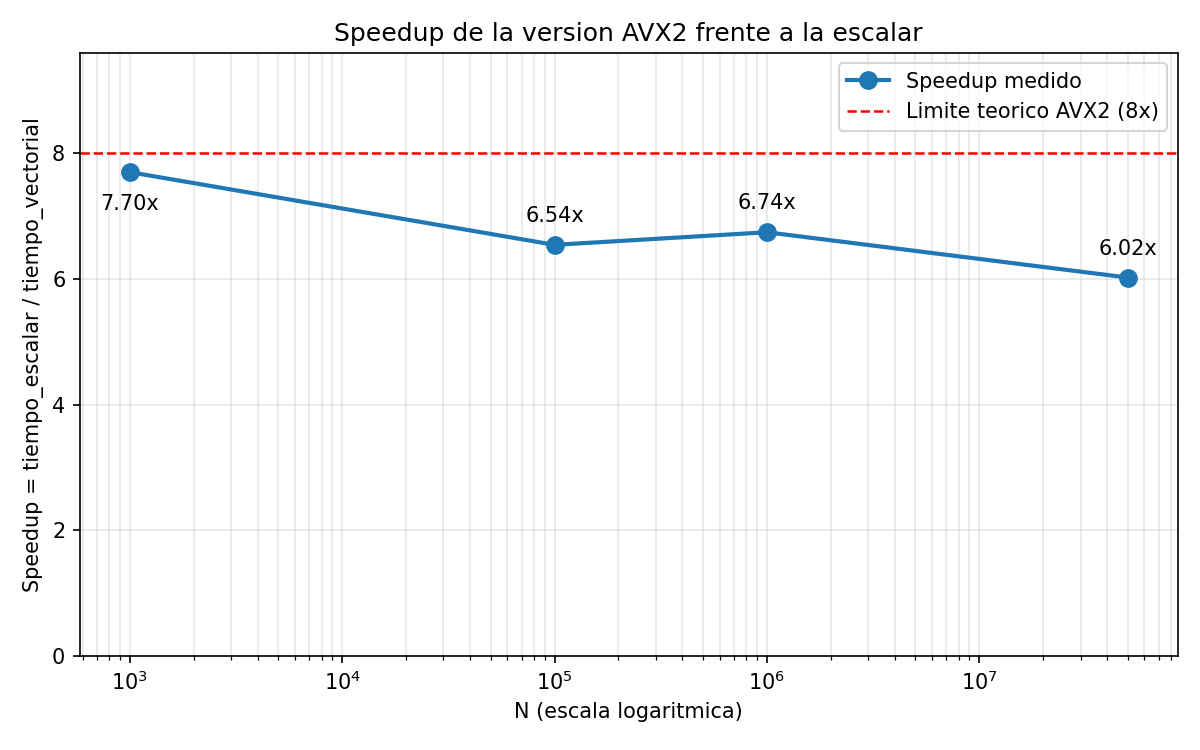
\includegraphics[width=\columnwidth]{fig/speedup.png}
  \caption{\textit{Speedup} de la versión AVX2 frente a la escalar en
           función de $N$ (eje horizontal logarítmico). La línea
           punteada marca el límite teórico de $8\times$ que impone el
           ancho de los registros YMM.}
  \label{fig:speedup}
\end{figure}

La Tabla~\ref{tab:fases} revela que \texttt{compute\_stats} se mantiene
entre $7,2$ y $8,3\times$ en todas las escalas, mientras que
\texttt{normalize\_array} cae de $7,75$ a $3,06\times$. Esto sucede por dos motivos: \texttt{normalize\_array} es la \textbf{única fase que escribe}, de modo que soporta el
doble de tráfico de memoria que las demás, y su bucle es el más
simple, con menos cómputo por byte transferido tras el que ocultar la
latencia. Es un caso directo de la ley de Amdahl: la fase que menos se
acelera termina dominando el tiempo total.

\subsection{Ciclos por elemento}

\begin{table}[ht]
\centering
\caption{Ciclos de referencia (TSC) por elemento procesado.}
\label{tab:ciclos}
\footnotesize
\begin{tabular}{|r|c|c|}
\hline
\textbf{N} & \textbf{Escalar} & \textbf{Vectorial} \\ \hline
$10^3$        & $26,850$ & $4,404$ \\ \hline
$10^5$        & $25,441$ & $3,425$ \\ \hline
$10^6$        & $24,743$ & $3,670$ \\ \hline
$5\times10^7$ & $24,598$ & $4,084$ \\ \hline
\end{tabular}
\end{table}

Esta métrica es especialmente informativa porque normaliza por la
cantidad de trabajo: es el costo de procesar un elemento, independiente de
cuántos haya. La versión escalar se mantiene \textbf{prácticamente
plana} (de $26,85$ a $24,60$), mientras que la vectorial alcanza su
mínimo en $N = 10^5$ y después \textbf{crece un \SI{19}{\percent}} hasta
$N = 5\times10^7$ haciendo exactamente el mismo trabajo por elemento.

La asimetría identifica el cuello de botella de cada versión. La
escalar está limitada por la \textbf{latencia} de su cadena de
dependencias: cada \texttt{addss} debe esperar el resultado del anterior,
y la compensación de Kahan alarga aún más esa cadena, de modo que
salir de la caché apenas la afecta porque ya estaba esperando. La
vectorial, mucho más rápida en cómputo, es la que sufre cuando los
datos dejan de llegar a tiempo.

\subsection{Contadores de hardware}

\begin{table}[ht]
\centering
\caption{Contadores de hardware, $N = 10^6$, 30 repeticiones.}
\label{tab:perf1e6}
\footnotesize
\setlength{\tabcolsep}{3pt}
\begin{tabular}{|l|r|r|c|}
\hline
\textbf{Métrica} & \textbf{Escalar} & \textbf{Vectorial} & \textbf{Razón} \\ \hline
\texttt{instructions}     & $1\,164,97$\,M & $148,08$\,M & $7,87\times$ \\ \hline
\texttt{cycles}           & $942,96$\,M    & $201,02$\,M & $4,69\times$ \\ \hline
IPC                       & $1,235$        & $0,737$     & --- \\ \hline
\texttt{cache-references}  & $22,41$\,M    & $15,95$\,M  & $1,41\times$ \\ \hline
\texttt{cache-misses}     & $13,74$\,M     & $9,30$\,M   & $1,48\times$ \\ \hline
Tasa de fallos            & \SI{61,3}{\percent}     & \SI{58,3}{\percent}  & --- \\ \hline
\end{tabular}
\end{table}

\begin{table}[ht]
\centering
\caption{Contadores de hardware, $N = 5\times10^7$, 20 repeticiones.}
\label{tab:perf5e7}
\footnotesize
\setlength{\tabcolsep}{3pt}
\begin{tabular}{|l|r|r|c|}
\hline
\textbf{Métrica} & \textbf{Escalar} & \textbf{Vectorial} & \textbf{Razón} \\ \hline
\texttt{instructions}     & $39\,714,29$\,M & $5\,240,23$\,M & $7,58\times$ \\ \hline
\texttt{cycles}           & $32\,263,41$\,M & $5\,861,95$\,M & $5,50\times$ \\ \hline
IPC                       & $1,231$         & $0,894$        & --- \\ \hline
\texttt{cache-references}  & $772,31$\,M    & $499,44$\,M    & $1,55\times$ \\ \hline
\texttt{cache-misses}     & $548,64$\,M     & $317,26$\,M    & $1,73\times$ \\ \hline
Tasa de fallos            & \SI{71,0}{\percent}      & \SI{63,5}{\percent}     & --- \\ \hline
\end{tabular}
\end{table}

\subsection{Discusión: cómputo o ancho de banda}

\textbf{El conteo de instrucciones confirma el beneficio teórico de
SIMD:} La versión vectorial ejecuta entre $7,58$ y $7,87$ veces
menos instrucciones que la escalar, muy cerca del límite de $8\times$
que impone el ancho de los registros YMM. La pequeña diferencia se
explica por el bucle de remanente y la reducción horizontal, que son
escalares. Es la métrica más limpia del beneficio de la vectorización
porque \textbf{no depende del reloj, de la caché ni de la carga del
sistema}; mide cuántas instrucciones hizo falta ejecutar para el mismo
trabajo. En instrucciones por elemento son $38,83$ frente a $4,94$ con
$N = 10^6$.

\textbf{La brecha entre instrucciones y ciclos mide el costo de la
memoria:} Si el cuello de botella fuera puramente de cómputo, ambas
razones coincidirían: ejecutar $7,87$ veces menos instrucciones
tomaría $7,87$ veces menos ciclos. Los ciclos, sin embargo, solo caen
$4,69\times$ con $N = 10^6$ y $5,50\times$ con $N = 5\times10^7$. Se
pierde así el \SI{40}{\percent} y el \SI{27}{\percent} del beneficio potencial respectivamente,
y esa pérdida es el tiempo que el procesador pasa esperando a la memoria
en lugar de calculando. \textbf{Esta es la explicación cuantitativa de
por qué el \textit{speedup} real no alcanza el $8\times$ teórico.}

\textbf{El IPC menor de la versión vectorial no indica ineficiencia:} El
IPC cuenta instrucciones completadas por ciclo, pero no todas las
instrucciones realizan el mismo trabajo, un \texttt{vaddps} procesa ocho
valores y un \texttt{addss} procesa uno. Comparar el IPC entre dos
versiones con distinto número de instrucciones es engañoso por
construcción. La métrica honesta es \textbf{elementos por ciclo}, con
$N = 10^6$, $0,0318$ para la escalar frente a $0,1492$ para la
vectorial. Un IPC bajo acompañado de muchas menos instrucciones totales
es precisamente la firma de un programa limitado por memoria.

\textbf{Los fallos de caché confirman la optimización no temporal:} El
tráfico teórico mínimo del algoritmo es de $0,3125$ líneas de
caché por elemento, cuatro recorridos de lectura más una escritura a
cuatro bytes por elemento en líneas de 64 bytes. Con
$N = 5\times10^7$ la versión vectorial mide $0,3173$ fallos por
elemento, apenas un \SI{1,5}{\percent} por encima de ese mínimo teórico: el
kernel accede a memoria de forma prácticamente óptima y no queda margen
de mejora en el patrón de acceso. La versión escalar mide $0,5486$,
un \SI{75}{\percent} por encima del mínimo, diferencia atribuible al \textit{read
for ownership} que \texttt{vmovntps} evita en la versión vectorial.


\textbf{Nota metodológica:} Una primera medición con solo 5
repeticiones sobre $N = 5\times10^7$ arrojó una razón de instrucciones
de $5,95\times$ en lugar de $7,58\times$. La discrepancia se debe a que
\texttt{perf stat} mide el \textbf{proceso completo}, incluida la lectura y
escritura de los \SI{191}{MB} del archivo, que es un costo fijo que no
escala con las repeticiones. Al aumentar a 20 repeticiones esa
contribución se diluye y la razón converge al valor esperado. El tiempo
de sistema reportado por \texttt{perf} ($0,478$s con 5 repeticiones
frente a $0,342$s con 20, mientras el trabajo útil se
cuadriplicaba) confirma la explicación. Por la misma razón, los
tiempos medidos bajo \texttt{perf} no son comparables con los de la
Tabla~\ref{tab:tiempos}, obtenidos sin instrumentación.

% =====================================================================
\section{Verificación con GDB}
\label{sec:gdb}

La sección 2.4, apartado a, inciso 3 del enunciado exige inspeccionar en tiempo de
depuración el contenido de un registro YMM inmediatamente después de
una instrucción \texttt{vaddps}, y el contenido de memoria del arreglo de
salida tras el bucle de normalización. La sesión se automatizó en
\texttt{tools/sesion\_gdb.txt} y se ejecuta con:

\begin{lstlisting}[style=shell]
$ python3 tools/gen_input.py 16 data/n16.dat random 42
$ gdb -x tools/sesion_gdb.txt --args ./bin/norm_vector \
      data/n16.dat data/o16.dat 1
\end{lstlisting}

Los puntos de ruptura se colocan sobre \textbf{etiquetas del ensamblador}
y no sobre números de línea, de modo que el guión sigue siendo
válido aunque el archivo se edite. GDB expone las etiquetas locales de
NASM con la forma \texttt{funcion.etiqueta}.

\subsection{Inspección del registro YMM}

Con $N = 16$ el bucle vectorial ejecuta exactamente dos iteraciones.

\begin{lstlisting}[style=shell,caption={Contenido de \texttt{ymm0} antes y
  después del \texttt{vaddps}.}, label={lst:gdb-ymm}]
Breakpoint 1, sum_array.sum_vec_loop ()
=> 0x555555556568 <sum_array.sum_vec_loop+9>:
       vaddps %ymm1,%ymm0,%ymm0

=== ITERACION 1: ANTES del vaddps ===
$1 = {0, 0, 0, 0, 0, 0, 0, 0}                 <- ymm0
$2 = {54.7912102, -12.2243118, 71.7195816,
      39.4736061, -81.1645279, 95.1244736,
      52.2279396, 57.2128601}                 <- ymm1

=== ITERACION 2: DESPUES del vaddps ===
$5 = {-19.5860634, -22.1471252, 45.8791885,
      124.826599, -52.3915024, 159.676788,
      40.910778, 2.66060257}                  <- ymm0
\end{lstlisting}

La verificación carril por carril confirma el modelo de ejecución. Los
elementos 8 a 15 de la entrada son $\{-74,3773$, $-9,9228$,
$-25,8404$, $85,3530$, $28,7730$, $64,5523$, $-11,3172$,
$-54,5523\}$, de modo que:
\begin{align*}
  \text{carril } 0 &: 54,7912 + (-74,3773) = -19,5861 \\
  \text{carril } 1 &: -12,2243 + (-9,9228) = -22,1471 \\
  \text{carril } 2 &: 71,7196 + (-25,8404) = 45,8792
\end{align*}
y así con los ocho. Cada carril $k$ acumula $\mathrm{arr}[k] +
\mathrm{arr}[k+8]$ de forma independiente: el registro \textbf{no contiene
un resultado sino ocho acumuladores separados}, que es precisamente el
modelo SIMD.

La suma de los ocho carriles vale $279,8293$, exactamente el valor que el
programa reporta como suma total. Esto verifica de forma independiente que
la reducción horizontal combina correctamente los carriles.

\subsection{Inspección de memoria y de la ABI}

\begin{lstlisting}[style=shell,caption={Argumentos recibidos y arreglo de
  salida tras el bucle de normalización.}, label={lst:gdb-mem}]
=== argumentos segun la ABI System V AMD64 ===
rdi (puntero in)  = 0x55555555b4c0
rsi (puntero out) = 0x55555555a480
edx (n)           = 16
$7 = 17.4893284      <- xmm0 = mean
$8 = 54.9311981      <- xmm1 = stddev
rsi mod 32 = 0       <- alineacion verificada

=== arreglo de salida (x/8fw) ===
0x55555555a480: 0.679065466  -0.540924668
                0.987239599   0.400214761
0x55555555a490: -1.79595304   1.41331601
                0.632402122   0.723150671
\end{lstlisting}

Esta captura verifica \textbf{en tiempo de ejecución} tres propiedades
afirmadas en la sección~\ref{sec:escalar}. Primero, la convención de
llamada: los dos punteros y el entero llegaron en \texttt{rdi},
\texttt{rsi} y \texttt{edx}, y los dos flotantes en \texttt{xmm0} y
\texttt{xmm1}, en una cola independiente. Segundo, la alineación:
$\texttt{rsi} \bmod 32 = 0$ confirma que \texttt{aligned\_alloc(32,\dots)}
cumplió y que \texttt{vmovaps} es seguro. Tercero, la correctud del
cálculo: $(54,7912 - 17,4893)/54,9312 = 0,679065$, que coincide
con el primer elemento del arreglo de salida hasta la novena cifra
significativa, diferencia atribuible al redondeo de \texttt{float32}.

Conviene señalar que las mediciones de tiempo que el \textit{driver}
reporta durante una sesión de GDB carecen de sentido, pues los puntos de
ruptura detienen el programa dentro de la región medida. Como indica el
propio enunciado, GDB es una herramienta de verificación funcional y de
inspección de bajo nivel, no de medición de tiempo.

% =====================================================================
\section{Precisión Numérica}
\label{sec:precision}

\subsection{Cancelación catastrófica en una sola pasada}
\label{sec:cancelacion}

La identidad $\mathrm{Var}(X) = E[X^2] - E[X]^2$ permitiría calcular la
varianza en un único recorrido. Se descartó por \textbf{cancelación
catastrófica}~\cite{goldberg1991}: la mantisa de 24 bits de
\texttt{float32} proporciona unos siete dígitos decimales significativos,
y cuando la media es grande respecto a la dispersión, $E[X^2]$ y
$E[X]^2$ son dos cantidades enormes y casi iguales; al restarlas los
dígitos significativos se cancelan y sobrevive únicamente el error de
redondeo.

\begin{table}[ht]
\centering
\caption{Varianza de $10^3$ valores alrededor de $10^6$ con dispersión
  $\pm 1$.}
\label{tab:cancelacion}
\footnotesize
\begin{tabular}{|l|r|c|}
\hline
\textbf{Método} & \textbf{Varianza} & \textbf{Error rel.} \\ \hline
Referencia (\texttt{float64})  & $0,340189$    & --- \\ \hline
Dos pasadas (\texttt{float32}) & $0,340219$    & $8,89\times10^{-5}$ \\ \hline
Una pasada $E[X^2]-E[X]^2$     & $-7\,077\,888$  & $2,08\times10^{7}$ \\ \hline
\end{tabular}
\end{table}

La versión de una pasada devuelve una varianza \textbf{negativa},
matemáticamente imposible. El método de dos pasadas evita el problema
porque la resta $x_i - \mu$ se realiza antes de elevar al cuadrado, de
modo que nunca se construyen las magnitudes enormes que después
habría que cancelar.

\subsection{Error de acumulación secuencial}
\label{sec:acumulacion}

Una implementación inicial con un único acumulador en \texttt{float32}
superó la tolerancia exigida a partir de $N = 10^6$. El diagnóstico es
directo: al acumular $\sum (x_i - \mu)^2$ sobre $10^6$ elementos el
acumulador alcanza un valor del orden de $3,3\times10^9$, y a esa
magnitud el espaciado entre dos \texttt{float32} consecutivos es de unos
400 unidades, mientras que cada término que se suma vale
aproximadamente 3300. El acumulador se vuelve tan grande respecto al
sumando que cada suma pierde bits bajos. El error crece como
$O(\sqrt{n}\,\varepsilon)$ en la práctica~\cite{higham2002}.

Un hallazgo relevante es que \textbf{la versión vectorial resultaba más
precisa que la escalar} sin ninguna medida adicional. La razón es que sus
ocho carriles constituyen ocho acumuladores independientes, cada uno con
$n/8$ términos, lo que equivale a una suma por bloques: con $N = 10^6$ el
error relativo de la varianza era de $3,55\times10^{-4}$ en la escalar
frente a $1,93\times10^{-5}$ en la vectorial, unas 18 veces mejor. La
vectorización, además de acelerar, mejoraba la exactitud.

Aun así, con $N = 5\times10^7$ también la versión vectorial fallaba
($5,53\times10^{-3}$), porque cada carril acumulaba $6,25\times10^6$
términos.

\subsection{Mitigaciones evaluadas}

Se consideraron cuatro alternativas:

\begin{enumerate}
  \item \textbf{Acumuladores parciales} mediante desenrollado del bucle,
        que reproduce en la versión escalar la ventaja de los carriles.
  \item \textbf{Suma por pares} (\textit{pairwise summation}), con error
        $O(\log n \cdot \varepsilon)$; es la que emplea \texttt{numpy.sum}
        internamente.
  \item \textbf{Suma compensada de Kahan}, con error $O(\varepsilon)$
        independiente de $n$, a costa de tres operaciones adicionales por
        elemento.
  \item \textbf{Acumulación en doble precisión}, que resuelve el
        problema pero contraviene el requisito de que todo el cómputo se
        realice en \texttt{float32}.
\end{enumerate}

Se adoptó la \textbf{suma compensada de Kahan}, porque es la única que
elimina la dependencia del error con $n$ sin abandonar la precisión
simple. La Tabla~\ref{tab:kahan} muestra que alcanza exactamente la misma
exactitud que acumular en doble precisión.

\begin{table}[h]
\centering
\caption{Error relativo de la varianza según la estrategia de
  acumulación.}
\label{tab:kahan}
\footnotesize
\setlength{\tabcolsep}{3pt}
\begin{tabular}{|l|c|c|}
\hline
\textbf{Estrategia} & $N = 10^6$ & $N = 5\times10^7$ \\ \hline
\texttt{float32}, un acumulador (escalar) & $3,55\times10^{-4}$ & --- \\ \hline
\texttt{float32}, 8 carriles (vectorial)  & $1,93\times10^{-5}$ & $5,53\times10^{-3}$ \\ \hline
Acumulación en \texttt{float64}          & $2,53\times10^{-8}$ & $2,74\times10^{-9}$ \\ \hline
\textbf{Kahan en \texttt{float32}}        & $\mathbf{2,53\times10^{-8}}$ & $\mathbf{2,74\times10^{-9}}$ \\ \hline
\end{tabular}
\end{table}

El costo es real y se cuantificó: la compensación de Kahan añade
cuatro operaciones por elemento y, más importante, \textbf{alarga la
cadena de dependencias serial} del bucle, ya que cada iteración necesita
la compensación de la anterior. La penalización medida fue de
aproximadamente un \SI{38}{\percent} en la versión escalar y un \SI{33}{\percent} en la
vectorial. Como ambas pagan un costo similar, el \textit{speedup} apenas
se altera: se ganó exactitud en cuatro órdenes de magnitud sin
modificar la conclusión sobre el beneficio de la vectorización.

\subsection{Interacción entre FMA y la compensación de Kahan}

El procesador soporta FMA, y una optimización aparentemente evidente
sería fusionar \texttt{vmulps} y \texttt{vaddps} en un \texttt{vfmadd}.
Se descartó por una razón de fondo: tras introducir la compensación
de Kahan, la resta del término de compensación queda \textbf{entre} la
multiplicación y la suma, de modo que no son fusionables directamente.
Más importante, la demostración de que la compensación de Kahan
captura exactamente el error de redondeo depende de que cada operación
redondee por separado según IEEE-754; el redondeo único de FMA
invalida ese supuesto y puede anular silenciosamente la compensación.

\subsection{Alcance de la compensación}

La suma compensada se aplica únicamente a la \textbf{pasada de
varianza}. \texttt{sum\_array} y la pasada de la media acumulan sin
compensación (un acumulador en la escalar, ocho carriles en la
vectorial). Hay dos razones. Primero, los términos de la varianza son
todos positivos y el acumulador crece hasta $\sim 10^9$, que es donde
se pierden bits; la suma de datos de media cercana a cero se mantiene
pequeña. Segundo, un error $\delta$ en $\mu$ afecta a la varianza solo
en segundo orden ($n\delta^2$), por la forma del algoritmo de dos
pasadas. La limitación es real: con datos de media grande y $N$
grande la suma sufriría el mismo problema de acumulación.

La compensación de Kahan cubre solo la varianza; la suma y la media
usan acumulación simple y podrían degradarse con datos de media grande.

% =====================================================================
\section{Conclusiones y Trabajo Futuro}
\label{sec:conclusiones}

\begin{itemize}
  \item La versión vectorizada con AVX2 alcanza un \textit{speedup} de
        $7,70\times$ con $N = 10^3$ que decrece monótonamente hasta
        $6,02\times$ con $N = 5\times10^7$. El decrecimiento se explica
        por el descenso del conjunto de trabajo a través de la jerarquía
        de memoria: con $N = 10^3$ cabe en L1, con $N = 10^5$ en L3, y con
        $N \ge 10^6$ excede toda la caché.

  \item \textbf{El \textit{speedup} no alcanza el $8\times$ teórico
        porque el cuello de botella se desplaza de cómputo a ancho de
        banda de memoria.} La evidencia es la brecha entre dos contadores
        de hardware: la versión vectorial ejecuta $7,58$ a $7,87$
        veces menos instrucciones ---prácticamente el límite del
        registro YMM--- pero consume solo $4,69$ a $5,50$ veces menos
        ciclos. Si el límite fuera el cómputo, ambas razones
        coincidirían.

  \item El análisis por fases identificó \texttt{normalize\_array} como
        el factor limitante: su \textit{speedup} cae hasta $3,06\times$
        mientras \texttt{compute\_stats} se mantiene sobre $7\times$. Es la
        única fase que escribe y por tanto la que soporta el doble de
        tráfico de memoria. Aplicar multiplicación por el recíproco y
        almacenamiento no temporal, seleccionados según el tamaño del
        arreglo, elevó su \textit{speedup} de $2,00$ a $3,06\times$
        con $N = 5\times10^7$.

  \item La acumulación secuencial en \texttt{float32} con un único
        acumulador excede la tolerancia exigida a partir de $N = 10^6$. La
        vectorización resulta \textbf{intrínsecamente más precisa}
        porque sus ocho carriles actúan como ocho acumuladores
        independientes, pero no basta en el tamaño mayor. La suma
        compensada de Kahan reduce el error a $2,74\times10^{-9}$ con
        $N = 5\times10^7$, igualando la exactitud de la doble precisión
        sin abandonar \texttt{float32}.

  \item Los fallos de caché de la versión vectorial ($0,3173$ por
        elemento) están a un \SI{1,5}{\percent} del mínimo teórico del
        algoritmo ($0,3125$), lo que indica que el patrón de acceso a
        memoria es prácticamente óptimo y que cualquier mejora adicional
        debería provenir de reducir el número de recorridos, no de
        acceder mejor.
\end{itemize}

\subsection{Limitaciones observadas}

El kernel realiza \textbf{cuatro recorridos de lectura} del arreglo por
ejecución: uno en \texttt{sum\_array}, dos en \texttt{compute\_stats}
(media y varianza) y uno en \texttt{normalize\_array}. En el régimen
limitado por memoria, ese número es el factor dominante del tiempo total.

La medición en tamaños pequeños presenta una dispersión elevada
inherente: con tiempos de kernel del orden de \SI{100}{\micro\second}, las
interrupciones periódicas del sistema operativo afectan a una fracción
apreciable de las muestras. El promedio permanece bien determinado (el
error estándar se mantiene por debajo del \SI{2}{\percent}) pero la desviación
muestral no es un buen indicador de calidad en ese régimen.

Finalmente, todas las mediciones se realizaron sobre una única
microarquitectura. Las latencias y \textit{throughputs} de instrucciones
como \texttt{vdivps}, así como la penalización de transición
AVX--SSE, son específicos de Skylake y podrían diferir en otras
generaciones.

\subsection{Trabajo futuro}

\begin{itemize}
  \item \textbf{Fusionar \texttt{sum\_array} con \texttt{compute\_stats}}
        para eliminar un recorrido completo del arreglo. Es la mejora de
        mayor impacto potencial en el régimen limitado por memoria, dado
        que reduciría el tráfico en un \SI{20}{\percent}.
  \item \textbf{Algoritmo de Welford}, que calcula media y varianza en una
        sola pasada de forma numéricamente estable. Se descartó aquí
        porque requiere una división por iteración y su
        vectorización no es directa, pero eliminaría otro recorrido.
  \item \textbf{Sustituir \texttt{vhaddps} por \texttt{vshufps} $+$
        \texttt{vaddps}} en la reducción horizontal, por consistencia con
        el enfoque ya empleado para mínimo y máximo.
  \item \textbf{Calibración más fina del umbral de almacenamiento no
        temporal.} Los datos de la Tabla~\ref{tab:calibracion} sugieren que
        el óptimo podría estar por debajo de los 393\,216 elementos
        derivados del tamaño de L3.
  \item \textbf{AVX-512} en hardware que lo soporte, evaluando el
        compromiso entre el doble de ancho vectorial y la posible
        reducción de frecuencia del núcleo.
\end{itemize}
\printbibliography
 
\end{document}